\documentclass[12pt] {report}
\usepackage[spanish]{babel}
\usepackage{natbib}
\usepackage{url}
\usepackage[utf8x]{inputenc}
\usepackage{amsmath}
\usepackage{graphicx}
\graphicspath{{images/}}
\usepackage{parskip}
\usepackage{fancyhdr}
\usepackage{vmargin}
\setmarginsrb{3 cm}{2.5 cm}{3 cm}{2.5 cm}{1 cm}{1.5 cm}{1 cm}{1.5 cm}

\title{Resultados de Investigación}				
\author{Br. Gerónimo Hernández Martínez}		

\date{\today}								

\makeatletter
\let\thetitle\@title
\let\theauthor\@author 
\let\thedate\@date
\makeatother

\pagestyle{fancy}
\fancyhf{}
\rhead{\theauthor}
\lhead{\thetitle}
\cfoot{\thepage}
\begin{document}

%%%%%%%%%%%%%%%%%%%%%%%%%%%%%%%%%%%%%%%%%%%%%%%%%%%%%%%%%%%%%%%%%%%%%%%%%%%%%%%%%%%%%%%%%

\begin{titlepage}
	\centering
    \vspace*{0.2 cm}
    
\includegraphics[scale = 0.60]{log1.png}\\[3.0 cm]
          \textsc{\LARGE Instituto Tecnologico Superior de Escarcega}\\[2.0 cm]	% University Name
	\textsc{\Large Estudio de detectores de rostros en sistemas de seguridad}\\[0.5 cm]				
	\textsc{\large Taller de Investigación II}\\[0.5 cm]				
	\rule{\linewidth}{0.2 mm} \\[0.4 cm]
	{ \huge \bfseries \thetitle}\\
    
	\rule{\linewidth}{0.2 mm} \\[1.5 cm]
	
	\begin{minipage}{0.4\textwidth}
		\begin{flushleft} \large
			\emph{Elaboró:}\\
			\theauthor
			\end{flushleft}
			\end{minipage}~
			\begin{minipage}{0.4\textwidth}
			\begin{flushright} \large
			\emph{Asesor:} \\
			Ing. Manuel Arturo Suarez Amendola,MC	
           
		\end{flushright}
        
	\end{minipage}\\[2 cm]
	
	{\large \thedate}\\[5 cm]
 
	\vfill
	
\end{titlepage}

%%%%%%%%%%%%%%%%%%%%%%%%%%%%%%%%%%%%%%%%%%%%%%%%%%%%%%%%%%%%%%%%%%%%%%%%%%%%%%%%%%%%%%%%%

\tableofcontents
\pagebreak

%%%%%%%%%%%%%%%%%%%%%%%%%%%%%%%%%%%%%%%%%%%%%%%%%%%%%%%%%%%%%%%%%%%%%%%%%%%%%%%%%%%%%%%%%

\section{Resumen}
En el presente trabajo  se pretende desmostar y dar resultados sobre la investigación realizada en el municipio de Escárcega sobre el estudio de detectores de rostros en sistemas de seguridad, en la cual se ha aplicado a una pequeña población de cinco empresas. Desde al inicio de la investigación se tomó en cuenta una de las siguientes  preguntas de investigación: ¿Cuál será el impacto en los sistemas de seguridad? Y ¿Cuál será el beneficio en las empresas que utilizan sistemas de seguridad?
Se utilizó como método para determinar si nuestra hipótesis es aceptada o rechazada una entrevista, en la cual se le aplicó a cinco empresas del municipio de Escárcega, estas empresas fueron analizadas y seleccionadas conforme a la necesidad o una problemática detectada, esto con el fin de poder ver la factibilidad de implementar el proyecto.
Al observar los datos obtenidos mediante la recolección de datos, se pudo decir la hipótesis fue parcialmente aceptada, ya algunas empresas elegidas para la aplicación de la entrevista no se pudo aplicar por motivos confidenciales, esto no permitió realizar un análisis más profundo en la investigación.
\textbf{\small Palabras clave: detectores de rostros, sistemas de seguridad, impacto, beneficio, factibilidad, hipótesis}.\\
\section{Abstract}

In the present work we intend to dismantle and give results on the investigation carried out in the municipality of Escárcega on the study of face detectors in security systems, in which it has been applied to a small population of five companies. Since the beginning of the research one of the following research questions was taken into account: What will be the impact on security systems? And what will be the benefit in companies that use security systems?
It was used as a method to determine if our hypothesis is accepted or rejected an interview, which was applied to five companies in the municipality of Escarcega, these companies were analyzed and selected according to the need or a problem detected, this in order to be able to see the feasibility of implementing the project.
Observing the data obtained through data collection, it was possible to say the hypothesis was partially accepted, and some companies chosen for the application of the interview could not be applied for confidential reasons, this did not allow a deeper analysis in the investigation.
\\

\textbf{\small Keywords: face detectors, safety systems, impact, benefit, feasibility, hypothesis}.

\section{Introducción}
Este trabajo está referido a un grupo de empresas privadas de seguridad en la cual manejan algún tipo de tecnología  de cámaras de vigilancia. El proyecto consiste en la investigación de la factibilidad de implementar sistemas de detectores de rostros a empresas, con la finalidad de que se pueda disminuir robos, mermas por parte de los empleados en empresas o poder evitar incidentes en establecimientos o instituciones, las personas encuestadas son dueños o gerentes, ya que se necesitaba informaciones de suma importancia y opiniones importantes para que este proyecto se lleve a cabo.

El robo de productos en las empresas es uno de los delitos que se han venido dando en cualquiera de las grandes y pequeñas empresas, y es rara vez que los delincuentes son atrapados y que han pagado por el delito, con la implementación de este sistema se pretende disminuir este tipo de actividades, esto con la ayuda de una cámara de seguridad con un sistema avanzado y una base de datos en la que se guardan imágenes de personas sospechosas y así al momento de detectar a una persona se iba a comparar con cuales correspondían a las que están almacenados en la base de datos, en caso de coincidir con alguna, se iba a mandar un mensaje al encargado de seguridad o a la gerencia.

El tipo de investigación que se realizó está basado en algunas investigaciones o proyectos realizados en países como España y Alemania en la cual es utilizada en sistemas de registros o de autentificación para el ingreso a un edificio o para algún software, este tipo de investigación se encuentra operando en varios lugares con el uso de visión por computadora o robótica, muchos países como Japón y china están muy enfocados en estos temas.

Uno de los alcances que nos llevará a la implementación de este proyecto es poder cubrir el trabajo del personal de seguridad en donde no se le dan accesos, este tipo de proyecto puede no solo implementarse en empresas, ya que es aplicable para sistemas policiacas, esto poder detectar a sospechosos que han sido identificados y almacenados en una base de datos, considero que servirá para poder tener un mayor control y seguridad en el municipio y de sus habitantes.

Me es importante mencionar que en el transcurso de la implementación el proyecto, es importante realizar un análisis del lugar en donde se realizara, ya que la importancia del lugar tiene mucho que ver, por la cantidad de iluminación.

El presente trabajo surge de los resultados obtenidos de una investigación realizada en la localidad de Escárcega, en donde se realizó una encuesta a cinco empresas que cuentan con tecnologías de cámaras de seguridad, para poder dar a conocer y ver la factibilidad sobre la implementación de sistemas de seguridad basadas en sistemas de detecciones de rostros. 

 



\section{Marco teórico}
(Cazorla Martínez, 2015) Menciona en su revista Software para la detección y el reconocimiento de rostros que:
“estas técnicas han evolucionado mucho, en dicha revista menciona dos de las técnicas para la implementación en un sistema capaz de detectar y reconocer rostros de personas introducidas previamente en el sistema.”


 \textbf{Fuentes de información }\\
Para realizar esta investigación considero que las empresas privadas como Bodega, Chedraui, Coppel e instituciones educativas brindarán informaciones suficientes, de igual forma las empresas de seguridad privada tales como CORDISUR, ya que la investigación les será de gran beneficio tanto en la economía de sus clientes  y en su sistema de seguridad.
Otra fuente de información es contactar algunas empresas en las que el investigador ha  trabajado tales como PAPRISA y SAPI en el municipio de Ciudad del Carmen.\\
\textbf{Factibilidad }\\
Considero que este proyecto es factible porque los resultados ayudara a las empresas implementar esta técnica en sus sistemas de seguridad, en la cual ayudara a disminuir el robo, identificando farderos, de igual forma reducir merma en empresas de servicios, en las instituciones permitirá el mayor control de sistemas de vigilancias.\\ 
1. OBJETIVOS DE LA INVESTIGACIÓN\\
1.1. OBJETIVO GENERAL    
\begin{itemize}
\item  Evaluar la factibilidad del servicio ofrecida en cada uno de las empresas en el Municipio Escárcega.
\end{itemize}

1.2. OBJETIVOS ESPECÍFICOS
\begin{itemize}
\item Identificar las necesidades de las empresas que manejan sistemas de seguridad en el Municipio Escárcega.
\item Determinar las expectativas de los gerentes de las empresas que manejan algún tipo de seguridad en el Municipio Escárcega.
\item Analizar la percepción de los gerentes con respecto al servicio ofrecido por las empresas en el Municipio Escárcega.
\end{itemize}

2. SISTEMA DE VARIABLE

2.1.- DEFINICIÓN NOMINAL
\\
Factibilidad  de servicio

2.2.- DEFINICIÓN CONCEPTUAL
La factibilidad del servicio expuesto  es el grado en el que gerente de cada uno de las empresas visitadas en la comunidad de Escárcega, se vea convencido en que su empresa requiera de estos servicios y vea una oportunidad de generar más ingresos a futuras y que ve la satisfacción de sus necesidades a través de los servicios que se le proporcionará. \\

 
2.3.- DEFINICIÓN OPERACIONAL

Cuadro 1
Operacionalización de la Variable

\textbf{Objetivo General:} Evaluar la factibilidad del servicio ofrecida en cada uno de las empresas en el municipio de Escárcega.
\begin{center}
    \begin{tabular}{ | p{3.5cm} | p{2cm}|  p{3cm} | p{5cm} |}
    \hline
    OBJETIVOS ESPECÍFICOS& VARIABLE & DIMENSIONES & INDICADORES \\ \hline
    -Identificar las necesidades de las empresas que manejan sistemas de seguridad en el municipio de Escárcega. &  & Necesidades de los gerentes de las empresas. & 
\begin{itemize}
\item Necesidad de poder disminuir perdidas en algunas áreas de mayor impacto.
\item Necesidad de reducir mermas.
\item Necesidad de garantizar la seguridad del personal en la que se trabaja.
\item Necesidad de vigilar y controlar el lugar o espacio de tra
\end{itemize}
bajo
 
 \\ \hline
    -Determinar las expectativas de los gerentes de las empresas que manejan algún tipo de seguridad en el Municipio Escárcega. & Factibilidad  de servicio & Expectativas de los gerentes de las empresas. & 
\begin{itemize}
\item Experiencias propias o en otras ramas del uso de las tecnologías.
\end{itemize}
 \\ \hline
    
    
    -Analizar la percepción de los gerentes con respecto al servicio ofrecido por las empresas en el municipio de Escárcega. & & Percepción de los gerentes de las empresas &
\begin{itemize}
\item Organización
\item Responsabilidad 
\item Seguridad
\item Confiabilidad
\end{itemize}
 \\
    \hline
       \end{tabular}
      
\end{center}
 Fuente: Elaboración propia


3. INFORMACIÓN ADICIONAL
3.1.-TIPO DE INVESTIGACIÓN
Cuantitativo y experimental 
Utilizar el enfoque cuantitativo y experimental ayudará a probar la las hipótesis que se planearán o a establecer nuevas ideas del proyecto, de igual forma considero que para este proyecto es necesario probar los resultados de la investigación, mediante la implementación de ello.\\

3.2. POBLACIÓN

Para esta investigación es de suma importancia realizar las entrevistas o encuestas con los gerentes generales de las empresas o a subgerentes, ya que la opinión de cada uno de ellos es de gran valor, y así poder asegurar o a resolver la hipótesis planteada.
Debido a que la población es pequeña se tomó una muestra de 5 empresas con las cuales cumplen con los requerimientos de la investigación.

\begin{center}
Cuadro 2
Características de la Población

\begin{tabular}{|c|c|}
	\hline 
	CARGO & SUJETOS \\ 
	\hline 
	A. Gerentes & 4 \\ 
	\hline 
	B. Subgerente  & 1 \\ 
	\hline 
	TOTAL & 5 \\ 
	\hline 
\end{tabular} 
 
Fuente: Elaboración propia
\end{center}

3.2.- INSTRUMENTO

Para la recolección de datos, se realizó una entrevista dirigida a cada uno de los gerentes de las empresas pertinentes de la ciudad de Escárcega conformada por diecisiete preguntas con respuestas en cada uno de sus apartados. (Anexo A) 

Para la recolección de datos, me es factible implementar una entrevista, con preguntas abiertas, ya que se logra entablar una conversación directa con el gerente de la empresa, y de igual forma permitirá anotar observaciones referentes a las hipótesis planteadas.\\
En el siguiente esquema se mostrará la bitácora de actividades, para la cual se llevó a cabo dicha investigación:
\begin{center}
			Bitácora de actividades \textbf{}
	\end{center}
\begin{center}
	\begin {tabular}{ | p{2cm} | p{11cm}|  }
	\hline
	\textbf {\begin{center}
			Fechas
	\end{center}}& \textbf{\begin{center}
	Actividades
\end{center}} \\ \hline
	17/02/2017 &  	
	\begin{itemize}
		\item Redacción del planteamiento del problema.
		\item 	Definición del tema de investigación.
		\item 	Elaboración de la pregunta de investigación.
	\end{itemize}
	
	
	\\ \hline
	24/02/2017 &	
	\begin{itemize}
		\item Ubicar las fuentes de información.
		\item 	Estudio de factibilidad.
		\item 	Definición de tipo de investigación.
		\item 	Elaboración de diagrama FODA.
		\item 	Análisis FODA
	\end{itemize}
	
	\\ \hline
	
	10/03/2017 & 	
	\begin{itemize}
		\item Redacción de marco teórico
	\end{itemize}
	.
	\\ \hline
	
	24/03/2017 & 
	\begin{itemize}
		\item Formulación de hipótesis del proyecto.
		\item Identificar variables.
	\end{itemize}
	\\ \hline
	
	27/03/2017 & 	
	\begin{itemize}
		\item Diseño y validación de los instrumentos de recolección de datos.
	\end{itemize}
	\\ \hline
	
	03/04/2017 & 	
	\begin{itemize}
		\item Recolección de datos.
	\end{itemize}
	\\ \hline
	
	24/04/2017 & 	
	\begin{itemize}
		\item Revisión de datos obtenidos.
	\end{itemize}
	\\ \hline
	
	08/05/2017 & 	
	\begin{itemize}
		\item Redacción de informe de investigación.
	\end{itemize}
	
	
	
	\\
	\hline
\end{tabular}

\end{center}
\newpage
\section{Conclusión}
Para concluir con este informe de investigación, es importante mencionar y agradecer a las empresas que nos dieron la oportunidad de poder ver y realizar la entrevista de manera formal, esta investigación puede tener un gran impacto en la sociedad si se llegara a aplicar o darle seguimiento como debe de ser, hoy en día las calles no cuentan con ningún tipo de seguridad ni vigilancia, es por ello que la realización de este proyecto implementado a hacia esa área puede funcionar, llevando un control sobre ellas, y de igual forma poder localizar y ubicar a las personas que cometen algún delito, y de esa manera también se puede buscar a personas desaparecidas o personas que están siendo buscadas por la ley, como se mencionó al principio, se pretende crear u obtener una base de daos en la cual estén almacenados las fotografías de cada una de las personas desaparecidas o que están siendo buscadas por algún delito.
En este proyecto de investigación se obtuvieron resultados no muy favorables, ya que las empresas están acostumbrados al modelo tradicional en la que han venido trabajando, de igual forma les costaría tiempo en adaptarse a este nuevo modelo tecnológico, mas sin embargo comentaron que en un futuro se podría requerir de este tipo de tecnologías.

\bibliographystyle{plain}
\bibliography{biblist}
 { Verificación de Identidad de Personas mediante. Sección de Electricidad y Electrónica}{62}
Balmelli Chuquisengo,  , L. E. (2006) ,

\ 
\\
{ Software para la detección y el reconocimiento de rostros. INGENIERÍA INFORMÁTICA}{10}
Cazorla Martínez,  ,R. (2015) ,

\ 
\\
{ DISEÑO DE UN SISTEMA DE RECONOCIMIENTO DE ROSTROS MEDIANTE LA HIBRIDACIÓN DE TÉCNICAS DE RECONOCIMIENTO DE PATRONES, VISIÓN ARTIFICIAL E IA, ENFOCADO A LA SEGURIDAD E INTERACCIÓN ROBÓTICA SOCIAL}{16-28}
Gualdrón, O. E., Duque Suárez, O. M., and Chacón Rojas, M. A. (Noviembre 2013) ,
\section{Anexo A}

\begin{figure}[!htb]
\caption{Primera hoja de la entrevista aplicada}
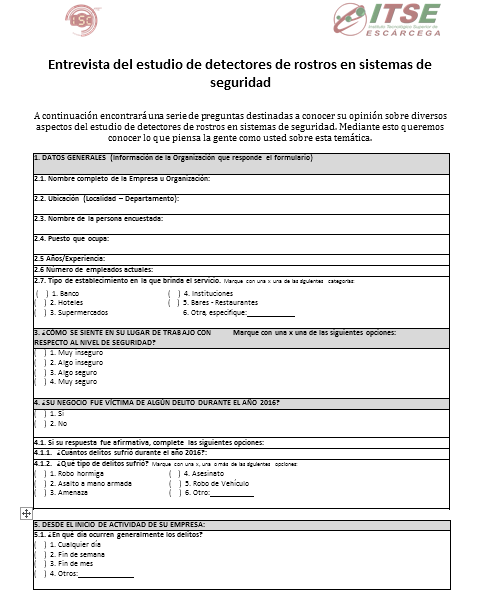
\includegraphics
[scale=1.3]{r1.PNG}
\end{figure}
\begin{figure}[!htb]
\caption{Segunda hoja de la entrevista aplicada}
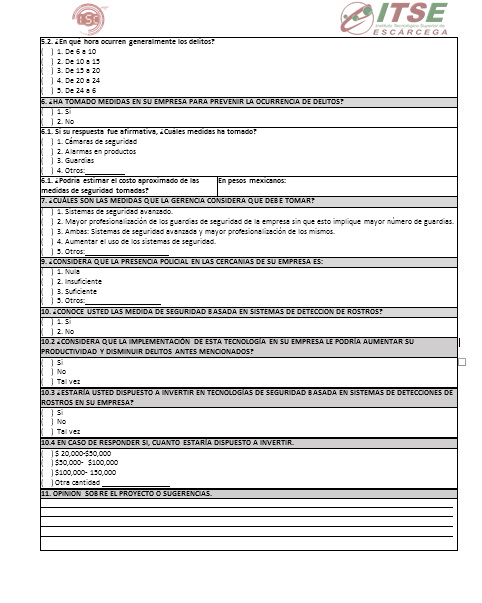
\includegraphics
[scale=1.3]{r2.PNG}
\end{figure}






\end{document}